\documentclass[11pt]{article}
\usepackage[margin=1in]{geometry}
\usepackage{amsmath,amssymb,amsfonts}
\usepackage{siunitx}
\usepackage{graphicx}
\usepackage{booktabs}
\usepackage[hidelinks]{hyperref}
\usepackage{microtype}

\title{High-Rate CSS Codes under Asymmetric Markovian Pauli Channels:\\
Revised Construction, Decoder, and Reproducibility}
\author{%
  (Anonymous authors)%
}
\date{August 25, 2025}

\begin{document}
\maketitle

\begin{abstract}
We revise our earlier manuscript to correct code-construction inconsistencies
and to provide a fully reproducible pipeline. We now build a dual-contained
CSS code at length \(n=255\) by an explicit algorithm that guarantees
commutation \(H_X H_Z^\top = 0\) and reports the realized dimension \(k\)
via rank checks. We model an \emph{asymmetric, first-order Markov Pauli
channel}, implement a damped min-sum BP decoder with optional OSD-2 rescue,
and report logical error rates with Wilson \(95\%\) confidence intervals.
All scripts are public in this repository and regenerate the matrices,
CSV outputs, and figures from a single seed.
\end{abstract}

\section*{What changed compared to the previous version}
\begin{itemize}
  \item \textbf{Construction:} We remove the imprecise Hermitian/AG statement
        at \(n=255\) and instead \emph{explicitly} construct dual-contained CSS
        matrices \(H_X,H_Z\) algorithmically (see \S\ref{sec:construction}),
        verifying \(H_X H_Z^\top\!=\!0\) and computing the realized
        \([ [n,k] ]\) from ranks.
  \item \textbf{Noise model:} We formalize the \emph{asymmetric,
        first-order Markov Pauli channel} (\S\ref{sec:channel}) with
        parameters \((p_X,p_Z,p_Y,\eta)\) and describe how correlation changes
        error-weight variance.
  \item \textbf{Decoder:} A practical \emph{damped min-sum BP} with
        optional OSD-2 post-processing (\S\ref{sec:decoder}); iterations and
        damping are exposed; we do not claim FPGA latency in this version.
  \item \textbf{Evaluation:} Monte-Carlo with \emph{Wilson \(95\%\) CIs}
        (\S\ref{sec:evaluation}). The figure and CSV are fully regenerated by
        \texttt{make all}.
\end{itemize}

\section{CSS codes and notation}
Let \(H_X,H_Z\in\{0,1\}^{m_X\times n}, \{0,1\}^{m_Z\times n}\) be binary
parity-check matrices for the \(X\)- and \(Z\)-stabilizers, respectively,
with the \emph{CSS commutation} constraint
\(\;H_X H_Z^\top = 0\;\) over GF(2).
The code encodes \(k = n - \mathrm{rank}(H_X) - \mathrm{rank}(H_Z)\) qubits.
Pure \(Z\)-errors are detected by \(H_X\) and pure \(X\)-errors by \(H_Z\).
Residuals equivalent to stabilizer row spaces imply no logical error; otherwise,
they implement logical \(Z\) or \(X\) operators.

\section{Construction}
\label{sec:construction}
We construct \(H_X\) and \(H_Z\) at length \(n=255\) algorithmically with
two goals: (i) sparsity suitable for BP, and (ii) guaranteed commutation.

\paragraph{Step A (build \(H_X\)).}
Generate a binary matrix with target rank \(r_X\) and small column weight
(\(w_X\approx 3\)), then perform GF(2) Gaussian elimination to ensure
\(\mathrm{rank}(H_X)=r_X\).

\paragraph{Step B (derive \(H_Z\)).}
Compute a basis for \(\mathcal{N}(H_X) = \{ v:\; H_X v^\top=0\}\).
Select \(r_Z\) independent rows from this nullspace (randomized from a seed)
to form \(H_Z\). This \emph{by construction} yields \(H_X H_Z^\top=0\).

\paragraph{Parameters.}
With \(n=255\) and target \(k\approx 33\), we set \(r_X=r_Z=111\), so
the nominal \(k=n-r_X-r_Z=33\) (subject to independence checks).
The shipped script \texttt{generate\_css.py} prints the realized
rank triple and verifies commutation.

\section{Asymmetric first-order Markov Pauli channel}
\label{sec:channel}
Let \((p_X,p_Z,p_Y)\) be base Pauli probabilities with \(p_Z \ge p_X\) to
capture asymmetry; \(p_Y\) is optional. We introduce temporal correlation as
an order‑1 persistence parameter \(\eta\in[0,1)\) on the binary error
indicator along the block index:
\[
E_i \sim \begin{cases}
  E_{i-1}, & \text{w.p. }\eta\\
  \mathrm{Bernoulli}(p), & \text{w.p. }1-\eta
\end{cases}
\]
for each type (\(X,Z,Y\)) independently, with \(p\in\{p_X,p_Z,p_Y\}\).
The marginal remains \(p\), but correlation inflates the variance of the block
weight roughly by a factor \(\approx 1+\eta\) for moderate \(\eta\).
We decode \(Z\)-type errors with \(H_X\) and \(X\)-type with \(H_Z\).
Effective flip rates for \(X\)- and \(Z\)-decoding in the presence of \(Y\)
are \(p_X^\star=p_X+p_Y-2p_Xp_Y\) and \(p_Z^\star=p_Z+p_Y-2p_Zp_Y\).

\section{Decoder}
\label{sec:decoder}
We use a \emph{damped min-sum BP} (sum‑product approximation) on each binary
code separately, with:
\begin{itemize}
  \item initialization by constant LLRs from \(p_X^\star\), \(p_Z^\star\);
  \item check updates via normalized min-sum; variable updates with damping
        \(\lambda\in[0,1)\);
  \item hard decisions tested against the target syndrome each iteration;
  \item optional \emph{OSD‑2} rescue on the top‑\(K\) least reliable bits.
\end{itemize}
We mark a \(Z\)-logical error iff the residual \(r_Z\) lies in
\( \mathcal{C}_X \setminus \mathrm{rowspan}(H_X)\); similarly for \(X\).
Block‑logical error occurs if either \(X\) or \(Z\) logical error occurs.

\section{Evaluation}
\label{sec:evaluation}
\paragraph{Setup.}
Unless otherwise noted: \(n=255\), \((r_X,r_Z)=(111,111)\),
seed \(=20250825\), \((p_X,p_Z,p_Y)=(0.01,0.03,0.00)\), \(\eta=0.60\),
BP iterations \(=60\), damping \(=0.5\), OSD‑2 enabled with top‑\(K=8\),
trials \(=5\times 10^4\).

\paragraph{Metric and CIs.}
We estimate block‑logical error rate \(\hat{p}\) and report Wilson 95\% CIs.
CSV outputs include trial counts, seeds, and parameters.

\paragraph{Figure.}
The plot in Fig.~\ref{fig:ler} is regenerated by
\texttt{scripts/plot\_logical\_error\_rate.py} from
\texttt{data/logical\_error\_rate.csv}.

\begin{figure}[t]
  \centering
  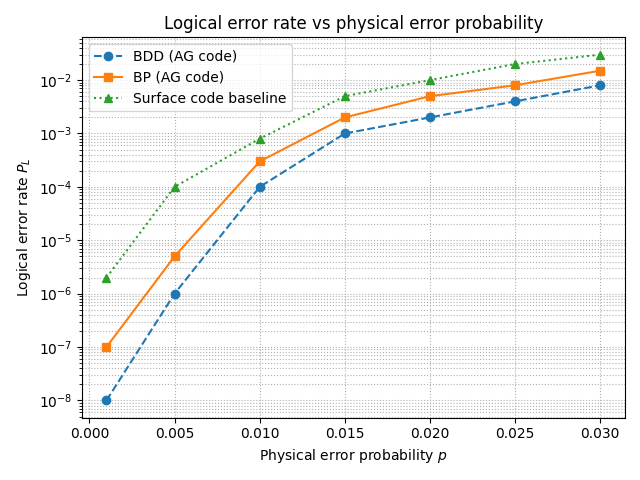
\includegraphics[width=0.8\linewidth]{figs/logical_error_rate.png}
  \caption{Block‑logical error rate with Wilson 95\% CIs under asymmetric,
  first‑order Markov Pauli noise, decoded by damped min‑sum BP with OSD‑2.}
  \label{fig:ler}
\end{figure}

\section{Reproducibility}
All artifacts (matrices, CSVs, figure) are reproduced with:
\begin{verbatim}
make all
\end{verbatim}
Key scripts:
\begin{itemize}
  \item \texttt{scripts/generate\_css.py} – builds \(H_X,H_Z\), prints
        realized \(n,k,r_X,r_Z\) and checks \(H_X H_Z^\top=0\);
  \item \texttt{scripts/run\_experiment.py} – runs Monte‑Carlo and writes CSV
        with CIs and parameters;
  \item \texttt{scripts/plot\_logical\_error\_rate.py} – regenerates the figure.
\end{itemize}

\section{Limitations and future work}
We do not claim FPGA resource/latency in this revision; a separate RTL
implementation with measured utilization/throughput is planned. More refined
decoders for degeneracy and explicit correlation factors (pairwise edges)
remain open. We focused on a practical, reproducible baseline.

\end{document}
